\chapter{Results and Discussion}

\section{Implementation Details}
All three system services run reproducibly from the repository root. The FastAPI backend initializes SQLite schema migrations, enforces \texttt{/24} IP masking on read routes via \texttt{mask\_ip\_for\_public()}, isolates seeded demo traffic under \texttt{demo: true}, and maintains hash-linked audit chains in \texttt{audit\_ledger}. A standalone builder script (\texttt{scripts/build\_public\_db.py}) produces the sanitized demonstration database (\texttt{data/public.db}) containing \textbf{9,320} masked devices with zero orphan alerts. On the frontend, the \texttt{/lab} Gate Explorer shares the exact TypeScript scoring port verified against Python golden vectors, while the Scenario Replay panel connects via WebSocket to stream tagged \texttt{demo: true} events in real time.

\begin{quote}
\textbf{[TODO — More / Screenshots]:} Capture and insert high-resolution PNG screenshots of the live running application (Windows/Kali local browser at \url{http://localhost:3000}): (1) \texttt{/} Hero \& Twin-Camera gate demo, (2) \texttt{/research} Real CUHK Avenue vs. Synthetic tables, (3) \texttt{/lab} Gate Explorer \& Scenario Replay streaming 12 demo alerts, (4) \texttt{/console} India map with \texttt{Simulated data active} banner, Inspector factors, and Ledger verify, and (5) \texttt{/ethics} passive scope statement. Save images inside \texttt{report/figures/} and embed here using figure floats.
\end{quote}

\section{Testing Strategies}
Software correctness and contract parity are guarded by two complementary automated suites executed across backend, video pipeline, evaluation harness, and frontend codebases:
\begin{enumerate}
  \item \textbf{Backend, Video Pipeline, and Evaluation Harness (\texttt{pytest}):} Verified \textbf{439 passed, 1 skipped, 0 warnings} across \texttt{backend/tests/}, \texttt{video\_pipeline/tests/}, and \texttt{eval/} (the single skip verifies the untrained-GNN 503 path cleanly when trained weights exist on disk). Unit and concurrency suites verify 50-request write locking without \texttt{SQLITE\_BUSY} failures, async event-loop cleanup, idempotency (409), clock-skew rejection (400), rate limiting (429), Merkle tamper detection, and strict refusal of unauthorized remote RTSP sources. Following the Docker-compatibility \texttt{ImportError} guard in \texttt{backend/routes/audit\_router.py}, \texttt{backend/tests/test\_gnn\_collusion\_model.py} passed (\texttt{16 passed, 1 skipped}).
  \item \textbf{Frontend Unit, Contract, and Build Verification (\texttt{Vitest}, \texttt{ESLint}, \texttt{TypeScript}):} All \textbf{11} Vitest suites (\textbf{81 passed} on Kali at commit \texttt{90f3265}) validate Python-vs-TypeScript gate parity on 265 golden test vectors, \texttt{/24} and IPv6 \texttt{/48} IP masking invariants, GeoJSON/TrustScore/WebSocket Zod contracts, SSE brief stream parsing, WCAG contrast ratios (12/12), brand SVG geometry, zero hard-coded numeric literals in section components, and generated SHA-256 sync with metric fixtures. Static verification confirms \texttt{npx eslint .} (0~errors, 0~warnings), \texttt{npx tsc --noEmit} (0~errors), and production \texttt{next build} completion across all routes.
\end{enumerate}

\textbf{[TODO — More / Manual \& E2E Testing]:} Add the manual cross-browser checklist across \texttt{/}, \texttt{/research}, \texttt{/lab}, \texttt{/console}, and \texttt{/ethics} tested against \texttt{90f3265} on two team laptops, plus Chromium Playwright E2E and \texttt{docker compose build} verification logs before final freeze.

\section{Result Analysis}
In accordance with Review~2 data hygiene, \textbf{real telemetry and real public video metrics} are reported completely independently from \textbf{synthetic formula verification checks}.

\subsection{Real India Exposure Aggregates (Censys Platform, Zero IPs)}
Under authorized research access (\texttt{RS-469}), \texttt{scripts/censys\_snapshot.py} stored aggregate metadata counts (zero raw IP addresses persisted or exported) matching \texttt{host.location.country: "India" AND host.services.hardware.type: "CAMERA"} in \texttt{data/censys/2026-11-26/snapshot.json}. Across India, Censys indexed \textbf{104,218} exposed camera hosts, of which \textbf{81,285} exposed RTSP port~554 alongside HTTP/HTTPS management ports across major Indian metropolitan centers, ASNs, and camera vendors. Multi-month longitudinal snapshots required to measure benign firmware turnover on the same hosts (Tier~1 field evaluation) are explicitly future scope.

\subsection{Real Public Video Evaluation (CUHK Avenue: Baseline \texttt{v1} vs. Tuned \texttt{v2})}
Tier~2 tamper detection was benchmarked on real public surveillance clips from the CUHK Avenue dataset resized to $320$~px width using reproducible programmatic tamper onset across eight attack categories (\texttt{eval/tier2\_real\_footage.py}). Clips shorter than $12$~s were excluded so tamper baselines could initialize ($14/16$ training videos retained = $0.1306$~h clean duration; $16/21$ held-out testing videos retained = $0.1195$~h clean duration). Tables~\ref{tab:avenue_train} and~\ref{tab:avenue_test} and Figures~\ref{fig:tripped_rates}--\ref{fig:fa_rates} compare the original detector (\texttt{v1}) against the tuned freeze-ring-buffer \texttt{v2} detector (\texttt{023c5c4}).

\begin{table}[!ht]
  \centering
  \caption{CUHK Avenue development set (\texttt{training\_videos}, $14$ clips, $0.1306$ clean hours): \texttt{v1} baseline vs. \texttt{v2} tuned}
  \label{tab:avenue_train}
  \begin{tabular}{@{}llccccc@{}}
    \toprule
    \textbf{Level} & \textbf{Scenario / Metric} & \textbf{v1 Hits} & \textbf{v1 Rate} & \textbf{v2 Hits} & \textbf{v2 Rate [95\% CI]} & \textbf{v2 Delay} \\
    \midrule
    tripped & freeze & 14/14 & 100.0\% & \textbf{14/14} & \textbf{100.0\%} [78.5, 100.0] & 1.00 s \\
    tripped & loop & 0/14 & 0.0\% & \textbf{14/14} & \textbf{100.0\%} [78.5, 100.0] & 0.56 s \\
    tripped & blur & 14/14 & 100.0\% & \textbf{14/14} & \textbf{100.0\%} [78.5, 100.0] & 0.00 s \\
    tripped & slow\_blur & 1/14 & 7.1\% & \textbf{14/14} & \textbf{100.0\%} [78.5, 100.0] & 5.94 s \\
    tripped & cover & 14/14 & 100.0\% & \textbf{14/14} & \textbf{100.0\%} [78.5, 100.0] & 0.00 s \\
    tripped & partial\_cover & 13/14 & 92.9\% & \textbf{14/14} & \textbf{100.0\%} [78.5, 100.0] & 0.76 s \\
    tripped & moved & 2/14 & 14.3\% & \textbf{14/14} & \textbf{100.0\%} [78.5, 100.0] & 1.96 s \\
    tripped & downscale & 14/14 & 100.0\% & \textbf{14/14} & \textbf{100.0\%} [78.5, 100.0] & 0.00 s \\
    \midrule
    tripped & Clean FA / hour & 6 FA & 45.9/h & \textbf{0 FA} & \textbf{0.0/h} [0.0, 28.2] & --- \\
    degraded & Clean FA / hour & 6 FA & 45.9/h & \textbf{0 FA} & \textbf{0.0/h} [0.0, 28.2] & --- \\
    \bottomrule
  \end{tabular}
\end{table}

\begin{table}[!ht]
  \centering
  \caption{CUHK Avenue held-out evaluation (\texttt{testing\_videos}, $16$ clips, $0.1195$ clean hours): \texttt{v1} vs. frozen \texttt{v2}}
  \label{tab:avenue_test}
  \begin{tabular}{@{}llccccc@{}}
    \toprule
    \textbf{Level} & \textbf{Scenario / Metric} & \textbf{v1 Hits} & \textbf{v1 Rate} & \textbf{v2 Hits} & \textbf{v2 Rate [95\% CI]} & \textbf{v2 Delay} \\
    \midrule
    tripped & freeze & 16/16 & 100.0\% & \textbf{16/16} & \textbf{100.0\%} [80.6, 100.0] & 1.00 s \\
    tripped & loop & 1/16 & 6.2\% & \textbf{15/16} & \textbf{93.8\%} [71.7, 98.9] & 0.56 s \\
    tripped & blur & 16/16 & 100.0\% & \textbf{16/16} & \textbf{100.0\%} [80.6, 100.0] & 0.00 s \\
    tripped & slow\_blur & 0/16 & 0.0\% & \textbf{16/16} & \textbf{100.0\%} [80.6, 100.0] & 5.88 s \\
    tripped & cover & 16/16 & 100.0\% & \textbf{16/16} & \textbf{100.0\%} [80.6, 100.0] & 0.00 s \\
    tripped & partial\_cover & 13/16 & 81.2\% & \textbf{16/16} & \textbf{100.0\%} [80.6, 100.0] & 0.76 s \\
    tripped & moved & 2/16 & 12.5\% & \textbf{16/16} & \textbf{100.0\%} [80.6, 100.0] & 1.96 s \\
    tripped & downscale & 16/16 & 100.0\% & \textbf{16/16} & \textbf{100.0\%} [80.6, 100.0] & 0.00 s \\
    \midrule
    tripped & Clean FA / hour & 4 FA & 33.5/h & \textbf{0 FA} & \textbf{0.0/h} [0.0, 30.9] & --- \\
    degraded & Clean FA / hour & 4 FA & 33.5/h & \textbf{1 FA} & \textbf{8.4/h} [0.2, 46.6] & --- \\
    \bottomrule
  \end{tabular}
\end{table}

On held-out test footage, \texttt{v2} dramatically closes the earlier detector blind spots: replay-loop detection improves from \textbf{1/16} (\texttt{6.2\%}) to \textbf{15/16} (\texttt{93.8\%}, median $0.56$~s), \texttt{slow\_blur} at \texttt{tripped} improves from \textbf{0/16} to \textbf{16/16} ($5.88$~s), \texttt{moved} improves from \textbf{2/16} to \textbf{16/16} ($1.96$~s), \texttt{partial\_cover} reaches \textbf{16/16} (speeding up median latency from $4.16$~s to $0.76$~s), and \texttt{tripped} clean false alarms drop from $33.5$/h ($4$ false alarms) to \textbf{0.0/h} ($0$ false alarms). Failure inspection highlights two honest edge bounds: held-out \texttt{video~13} ($14.3$~s short clip, minimum score $0.986$) missed \texttt{loop} detection, and \texttt{video~06} ($41.3$~s) generated one transient \texttt{degraded} warning ($2.61\%$ of clip duration) without tripping the hard gate. Moreover, because un-tampered held-out duration totals $0.1195$~h ($\approx 7.2$~minutes), the exact Poisson 95\% upper confidence bound on zero false alarms sits at \textbf{30.9/h} ($30.876$/h), underscoring the need for longer clean field streams.

\begin{figure}[!ht]
  \centering
  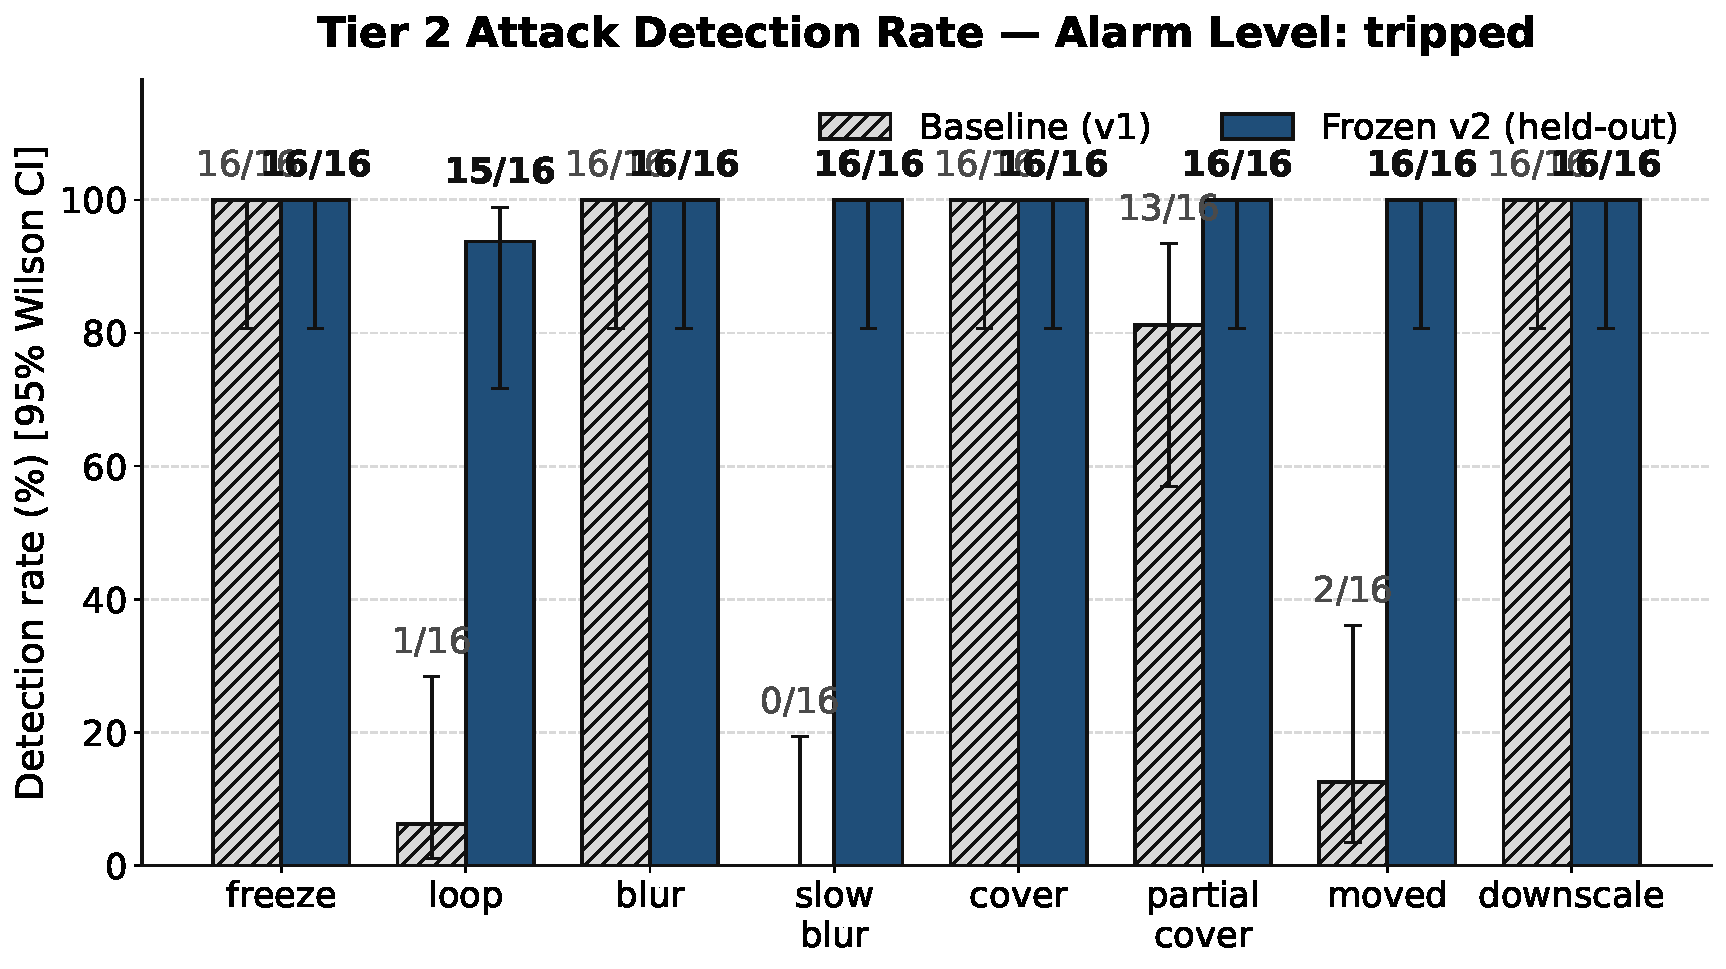
\includegraphics[width=0.92\textwidth]{detection_rate_tripped.pdf}
  \caption{Real CUHK Avenue held-out detection rate comparison at the \texttt{tripped} threshold (\texttt{v1} baseline vs. \texttt{v2} tuned)}
  \label{fig:tripped_rates}
\end{figure}

\begin{figure}[!ht]
  \centering
  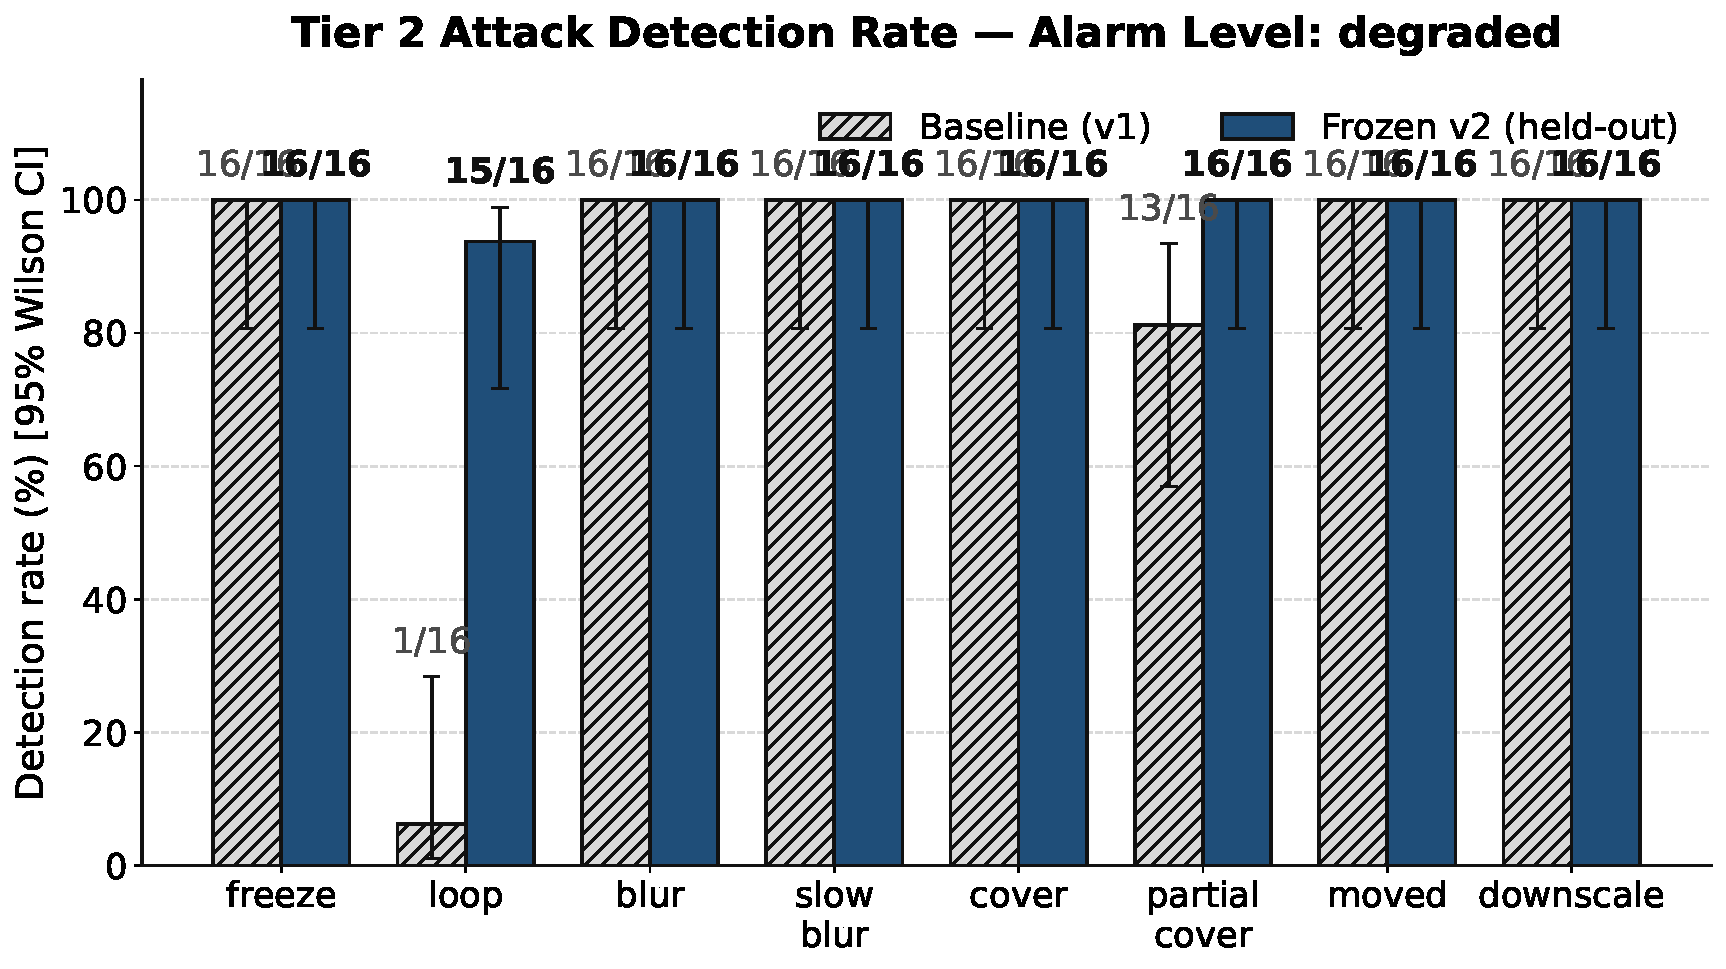
\includegraphics[width=0.92\textwidth]{detection_rate_degraded.pdf}
  \caption{Real CUHK Avenue held-out detection rate comparison at the early \texttt{degraded} warning level}
  \label{fig:degraded_rates}
\end{figure}

\begin{figure}[!ht]
  \centering
  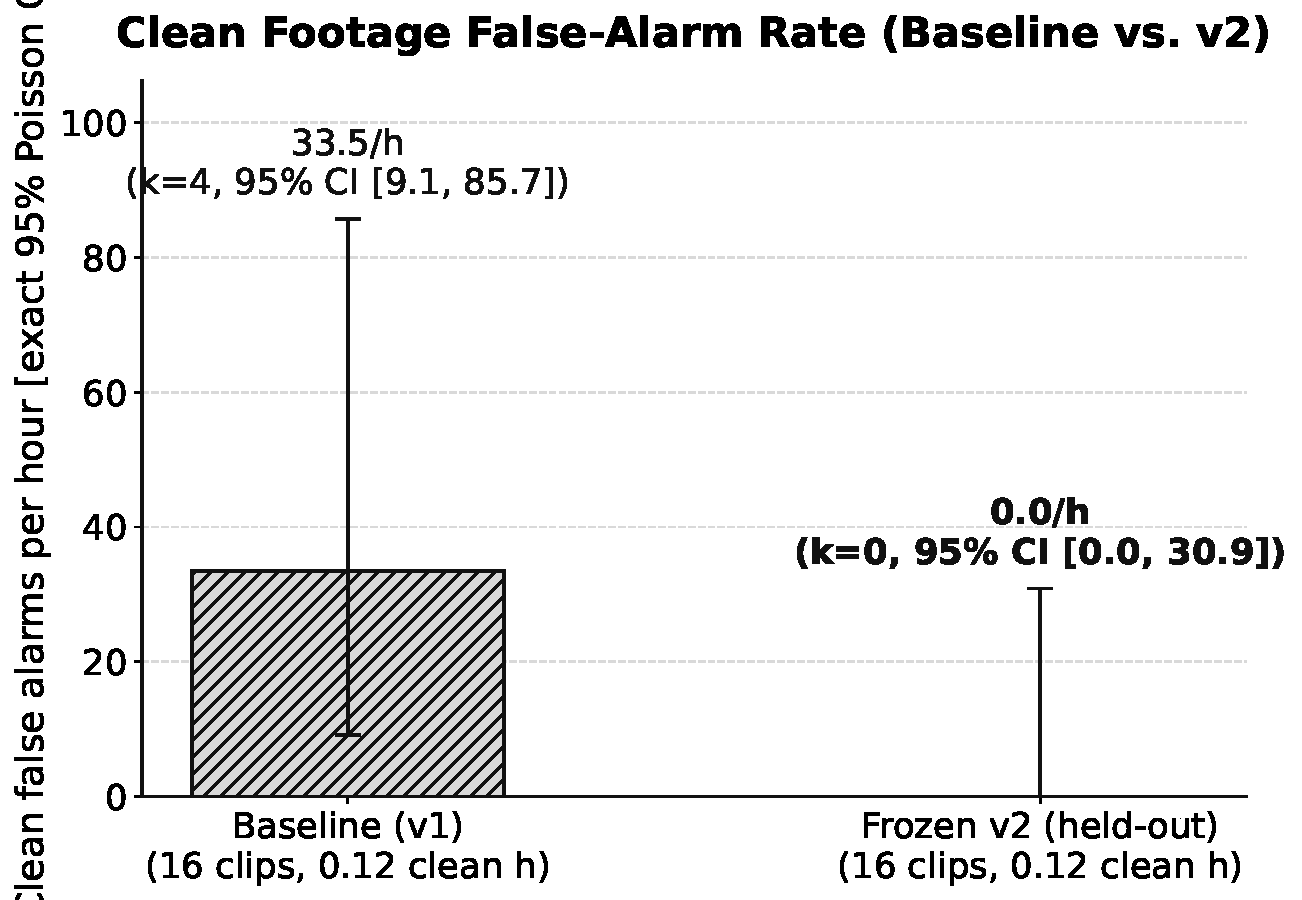
\includegraphics[width=0.78\textwidth]{false_alarms_per_hour.pdf}
  \caption{Clean-footage false alarm rates per hour (with exact 95\% Poisson confidence bounds) on Avenue training and held-out sets}
  \label{fig:fa_rates}
\end{figure}

\subsection{Runtime CPU Throughput Benchmark}
Timed across 300 frames (\texttt{synthetic\_pattern} $320 \times 180$) on an Intel Core i5-12450H CPU using Python~3.12.6 and OpenCV~5.0.0 (\texttt{eval/benchmark\_speed.py}), \texttt{v2} sustains \textbf{281.9~FPS} ($3.55$~ms/frame) at $320$~px width and \textbf{71.2~FPS} ($14.04$~ms/frame) at $640$~px width against \texttt{v1}'s $606.8$~FPS and $84.8$~FPS. Thus, even with full ring-buffer loop checks enabled on CPU alone, \texttt{v2} maintains more than $2\times$ real-time throughput headroom above standard $25\text{--}30$~FPS IP camera streams. Pure-Python IG-DCTF fusion adds minimal overhead ($4.69~\mu$s/call vs. $2.60~\mu$s/call for Channel~A alone, excluding I/O).

\subsection{Synthetic Formula Sanity Check and Ablation (\texorpdfstring{$n = 120$}{n = 120}, Explicitly Labelled Synthetic)}
To verify that the IG-DCTF equation obeys non-compensation and does not degrade posture scoring when Channel~B telemetry is absent, Table~\ref{tab:syn_models} and Figures~\ref{fig:syn_cmp}--\ref{fig:decision_map} summarize results across $120$ hand-authored scenarios ($63$ fabricated, $57$ genuine; $30$ containing Channel~B drift/liveness values, $90$ carrying attribute posture only).

\begin{table}[!ht]
  \centering
  \caption{Synthetic formula sanity check ($n = 120$, positive = \texttt{fabricated}; \textbf{synthetic corpus, not field accuracy})}
  \label{tab:syn_models}
  \begin{tabular}{@{}lccccccccc@{}}
    \toprule
    \textbf{Model / Variant} & \textbf{Acc.} & \textbf{Prec.} & \textbf{Recall} & \textbf{Spec.} & \textbf{$F_1$} & \textbf{TP} & \textbf{FP} & \textbf{TN} & \textbf{FN} \\
    \midrule
    Weighted Average (WA) & 0.7917 & 1.0000 & 0.6032 & 1.0000 & 0.7525 & 38 & 0 & 57 & 25 \\
    Advanced (Channel~A only) & 0.8333 & 1.0000 & 0.6825 & 1.0000 & 0.8113 & 43 & 0 & 57 & 20 \\
    Bayesian Log-Odds & 0.8417 & 0.9400 & 0.7460 & 0.9474 & 0.8319 & 47 & 3 & 54 & 16 \\
    Channel~B only & 0.6250 & 1.0000 & 0.2857 & 1.0000 & 0.4444 & 18 & 0 & 57 & 45 \\
    Additive fusion ($T_{\mathrm{cve}} - 70(1-s)$) & 0.9167 & 1.0000 & 0.8413 & 1.0000 & 0.9138 & 53 & 0 & 57 & 10 \\
    \textbf{IG-DCTF (Multiplicative Gate)} & \textbf{0.9750} & \textbf{1.0000} & \textbf{0.9524} & \textbf{1.0000} & \textbf{0.9756} & \textbf{60} & \textbf{0} & \textbf{57} & \textbf{3} \\
    \bottomrule
  \end{tabular}
\end{table}

Stratification confirms the gate acts selectively: on the $n = 90$ scenarios without Channel~B signals, IG-DCTF identically matches Channel~A ($0.967$ accuracy / $0.966$ $F_1$), whereas on the $n = 30$ Channel-B scenarios, vulnerability-only models sit near chance ($0.433$--$0.467$ accuracy) while IG-DCTF attains $1.000$ (exact McNemar~\cite{mcnemar1947} $17$ vs. $0$ discordant scenarios, $p = 1.53 \times 10^{-5}$). Additive fusion misses $10$ attacks versus $3$ for the multiplicative gate, proving why non-compensation matters. Across 42 threshold pairs, the sweep surface stays flat ($0.9756$ $F_1$ everywhere), meaning thresholds $(0.50, 0.85)$ are justified analytically rather than fitted on data. Synthetic Tier~1 ($13$ distinct drift pairs, $0.0038$~ms/device) and earlier synthetic Tier~2 checks ($80$ runs, $9.6$~frames mean latency) provide regression checks rather than field estimates.

\begin{figure}[!ht]
  \centering
  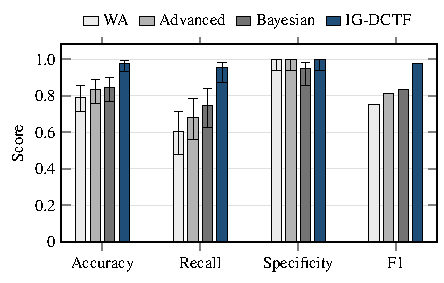
\includegraphics[width=0.88\textwidth]{fig08_comparison.pdf}
  \caption{Synthetic 120-scenario comparison across WA, CVE-only (Advanced), Bayesian, and IG-DCTF (with 95\% Wilson~\cite{wilson1927} bounds)}
  \label{fig:syn_cmp}
\end{figure}

\begin{figure}[!ht]
  \centering
  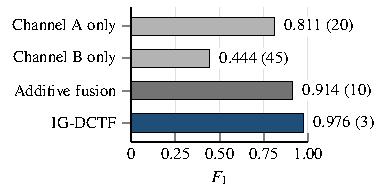
\includegraphics[width=0.78\textwidth]{fig09_ablation.pdf}
  \caption{Ablation on synthetic corpus showing why multiplicative gating avoids linear compensation ($FN = 3$ vs. $10$ additive)}
  \label{fig:ablation}
\end{figure}

\begin{figure}[!ht]
  \centering
  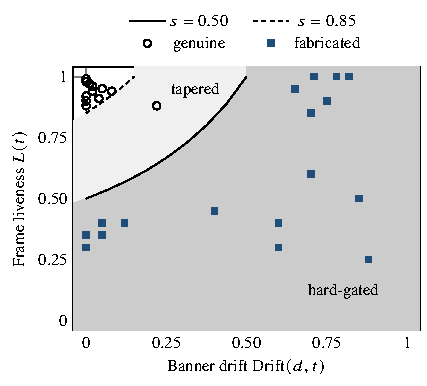
\includegraphics[width=0.72\textwidth]{fig10_decision_map.pdf}
  \caption{IG-DCTF decision regions in the $(\mathrm{Drift}, L)$ plane showing iso-integrity curves at $s = 0.50$ and $s = 0.85$}
  \label{fig:decision_map}
\end{figure}
